%% LyX 2.3.4.2 created this file.  For more info, see http://www.lyx.org/.
%% Do not edit unless you really know what you are doing.
\documentclass[english]{article}
\usepackage[T1]{fontenc}
\usepackage[latin9]{luainputenc}
\usepackage{float}
\usepackage{booktabs}
\usepackage{graphicx}
\usepackage[authoryear]{natbib}

\makeatletter

%%%%%%%%%%%%%%%%%%%%%%%%%%%%%% LyX specific LaTeX commands.
%% Special footnote code from the package 'stblftnt.sty'
%% Author: Robin Fairbairns -- Last revised Dec 13 1996
\let\SF@@footnote\footnote
\def\footnote{\ifx\protect\@typeset@protect
    \expandafter\SF@@footnote
  \else
    \expandafter\SF@gobble@opt
  \fi
}
\expandafter\def\csname SF@gobble@opt \endcsname{\@ifnextchar[%]
  \SF@gobble@twobracket
  \@gobble
}
\edef\SF@gobble@opt{\noexpand\protect
  \expandafter\noexpand\csname SF@gobble@opt \endcsname}
\def\SF@gobble@twobracket[#1]#2{}
%% Because html converters don't know tabularnewline
\providecommand{\tabularnewline}{\\}

%%%%%%%%%%%%%%%%%%%%%%%%%%%%%% Textclass specific LaTeX commands.
\newenvironment{lyxlist}[1]
	{\begin{list}{}
		{\settowidth{\labelwidth}{#1}
		 \setlength{\leftmargin}{\labelwidth}
		 \addtolength{\leftmargin}{\labelsep}
		 \renewcommand{\makelabel}[1]{##1\hfil}}}
	{\end{list}}

%%%%%%%%%%%%%%%%%%%%%%%%%%%%%% User specified LaTeX commands.
\usepackage{babel}

\makeatother

\usepackage{babel}
\begin{document}
\title{Hello}
\author{Srdjan Tijanic}
\maketitle
\begin{abstract}
This is so cool and easy to use. It took me some time to figure out
but I am so pleased now. It is so pretty that I decided to keep it.

\section{Introduction}

This is an example of an inline equation: $E=mc^{2}$\footnote{This is Einstein}.

\section{Experiment\protect\protect\footnote{This is Newton, at least the apple.}}

Definitely everything looks nice today. Check in chapter: \ref{sec:Inline-table}.

\begin{figure}[h]
\begin{centering}
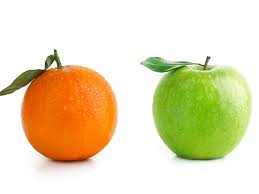
\includegraphics[scale=0.5,viewport=0bp 0bp 259bp 194bp]{example-image.jpeg} 
\par\end{centering}
\caption{Something better than other}
\end{figure}
\end{abstract}
\newpage{}

\section{Inline table\label{sec:Inline-table}}
\begin{verbatim}
And it's getting better and better!!!
\end{verbatim}
\noindent 
\begin{table}[H]
\begin{centering}
\begin{tabular}{ccccc}
\toprule 
a  & b  & c  & d  & e\tabularnewline
\midrule
\midrule 
1  &  &  &  & 1\tabularnewline
\midrule 
 & 1  &  &  & \tabularnewline
\midrule 
 &  & 1  &  & \tabularnewline
\midrule 
 &  &  & 1  & \tabularnewline
\bottomrule
\end{tabular}
\par\end{centering}
\centering{}\caption{Cool table, isn't it?}
\end{table}

\bigskip
\bigskip
\bigskip

\section{Conclusion}

I hope this will make a difference! 
\begin{lyxlist}{00.00.0000}
\item [{Version:}] 90bdf5af3be271b3294f0b8bcfb1a80056acdcfb 
\end{lyxlist}

\end{document}
